\documentclass[table,xcdraw]{beamer}
\usetheme{Madrid}

\usepackage[utf8]{inputenc}
\usepackage{default}
\usepackage[T1]{fontenc}
\usepackage{wrapfig}
\usepackage[export]{adjustbox}
\usepackage{wrapfig}
\usepackage{verbatim}

\begin{document}

\title[MaldOS] % (optional, only for long titles)
{{\huge\textsc{MaldOS}:} \\
a Moderately Abstracted Layer for Developing Operating Systems}
\author[Mattia Maldini] % (optional, for multiple authors)
{Mattia Maldini\\[3mm]Relatore: Renzo Davoli\\[3mm]}

\institute[Università di Bologna] % (optional)
{
  Università di Bologna
}
\date[Laurea 2019] % (optional)
{Sessione di laurea 14 marzo 2019}
\subject{Informatica}

\frame{\titlepage}

\begin{frame}[fragile]
    Structuring an Operating Systems course can be a thorny task. \\
    \bigskip
    Topics like
    scheduling, parallel programming, virtual memory and context switching are 
    hard to grasp via a purely abstract approach, and developing a concrete 
    example is inherently non trivial.\\
    \bigskip
    A previous solution to this issue was the $\mu$MPS family of emulators; this
    work proposes a slight shift in the form of an abstraction layer allowing for
    easier development on real hardware.
    \begin{comment}
        I sistemi operativi sono un argomento particolarmente spinoso nel contesto
        dell'insegnamento. I concetti che vengono coperti possono essere facilmente
        compresi a un livello superficiale e intuitivo, ma sono difficili da 
        interiorizzare senza un approccio pratico; approccio pratico che, considerata
        l'inerente complessita' dell'argomento, e' a sua volta complesso da
        applicare.
        Una soluzione seguita nel corso degli anni dal professor Davoli si appoggia
        a uMPS e simili, una famiglia di emulatori ad hoc per architettura MIPS 
        (e ARM).
        MaldOS e' una variazione sul tema; e' un acronimo per Moderately
        Abstracted Layer for Developing Operating Systems, ovvero un layer
        che renda piu' semplice (ma non troppo) l'approccio all'hardware di
        una architettura reale.
    \end{comment}
\end{frame}

\begin{frame}[fragile]
    \frametitle{Tradeoffs}
    $\mu$MPS2 allows students to work in a simplified environment while still being
    faithful to the real MIPS architecture, providing an interesting experience.
    However
    \begin{itemize}
        \item it is still abstract work, as the resulting OS will never run on a real device
        \item $\mu$MPS is an ad-hoc emulator
        \item Its debugging facilities lack step-by-step execution of C code
        \item MIPS is a dated architecture
    \end{itemize}
    \begin{comment}
        uMPS riproduce fedelmente un'architettura reale, offrendo quindi un
        esempio didatticamente interessante, rimuovendo i dettagli che non
        sono interessanti per lo studio dei sistemi operativi. Per esempio, 
        l'interazione con le periferiche tramite registri e' considerata parte
        integrante dello sviluppo di un sistema operativo; l'elevata complessita'
        dei protocolli di controllo di suddette periferiche e' invece un ostacolo
        all'apprendimento.
        uMPS cerca quindi di trovare un equilibrio tra un lavoro concreto (e quindi interessante)
        e un ambiente virtuale piu' accessibile per gli studenti. Riesce in questo
        obbiettivo, ma con alcuni caveat:
        Pur appoggiandosi a un'architettura reale, la macchina uMPS e' comunque
        astratta e inesistente; il lavoro sviluppato non trova quindi corrispondenze
        al di fuori dell'emulatore.
        Per quanto sia un tool ben sviluppato si tratta di un progetto accademico
        di nicchia; gli studenti imparano ad usarlo e lo dimenticano dopo l'esame.
        Offre delle visualizzazioni di debug specifiche e sofisticate, ma ha il
        grande difetto di non permettere l'esecuzione step-by-step del codice C.
        Infine, MIPS e' un'architettura ormai datata, e per gli studenti puo'
        essere piu' interessante studiare ambienti piu' moderni e diffusi, come ARM.
    \end{comment}
\end{frame}

\begin{frame}[fragile]
    \frametitle{Tradeoffs}
    \textbf{MaldOS} is an abstraction layer devised to reproduce an $\mu$MPS-like simplified
    environment on a real device and architecture, the Raspberry Pi 3 and ARMv8.
    \begin{itemize}
        \item it is an extremely practical example, and the result can be run on a real machine
        \item it relies on general purpose software (namely, Qemu and GDB)
        \item its debugging facilities are less specific but more powerfull (full GDB support)
        \item ARM is a more modern and widespread environment
    \end{itemize}
    \begin{comment}
        Rispetto a quando uMPS e' stato concepito, l'architettura ARM presenta 
        un'opportunita' piu' interessante ai fini di un progetto accademico. In 
        particolare, il layer di astrazione e' pensato per girare su un Raspberry Pi 3,
        una board educativa largamente diffusa; in questo modo gli studenti possono
        avere la soddisfazione di vedere il proprio lavoro eseguito su una macchina
        reale.
        L'hardware da solo sarebbe un ambiente di sviluppo inclemente; serve comunque
        un emulatore. Trattandosi di un dispositivo diffuso ci si puo' avvalere 
        di Qemu, che ha recentemente supportato anche il modello 3. Lavorando su
        un emulatore general purpose si ottengono tutti i benefici del caso, tra
        cui il pieno supporto di GDB.
        ARMv8 e' una architettura moderna e 
    \end{comment}
\end{frame}

\begin{frame}[fragile]
    \frametitle{Bare Metal}
    The problem with a real architecture is the intrinsic complexity of hardware
    management. The abstraction layer softens the approach by partially taking care 
    of initialization and configuration procedures.
    \begin{figure}[b]
    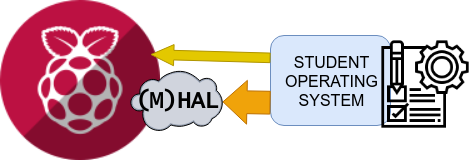
\includegraphics[scale=0.7]{raspberrypi.png}
    \end{figure}
    \begin{comment}
        Come gia' detto, l'astrazione deve essere soltanto parziale; alcuni tratti
        dell'hardware, del "bare metal development" sono considerati parte integrante
        dell'esperienza; altri sono soltanto un fastidio. Seguendo questa filosofia,
        per esempio,
        gli studenti si troveranno a interagire con uno spazio di memoria nudo
        e senza protezioni dove definire gli interrupt handler, ma gli verra'
        risparmiato lo sforzo di doverli creare in linguaggio Assembler.
        In generale il layer di astrazione si occupa di quattro aspetti.
    \end{comment}
\end{frame}

\begin{frame}[fragile]
    \frametitle{Initialization}
    \begin{itemize}
        \item A proper linker script is setup beforehand
        \item Move to the correct level of execution
        \item Prepare memory structure (stack pointers and such)
        \item Boot all four kernels and park three
        \item Prepare the C environment (zero bss section)
        \item Configure and initialize all real devices (UART, screen, SD)
    \end{itemize}

    \begin{comment}
        Il primo e' l'inizializzazione. Prima ancora di 
        eseguire il programma e' necessario organizzare adeguatamente la memoria
        tramite un linker script che posizioni il kernel a un certo indirizzo e
        ponga le basi per l'esecuzione.
        Le prime operazioni riguardano la configurazione dei registri di sistema
        e lo spostamento al livello di esecuzione corretto; dopodiche' bisogna
        preparare stack pointer e interrupt handler per i livelli di esecuzione
        interessati. Inizialmente soltanto uno dei quattro core e' attivo: gli
        altri tre devono essere svegliati e messi in pausa, pronti per lavorare.
        Fino a questo punto non c'e' un ambiente C completo, e si deve lavorare
        in Assembler; da qui si inizializza
        la sezione .bss delle variabili globali e si passa il controllo a una
        routine C che passa a configurare tutti i dispositivi.
        Solo dopo tutte queste preparazioni si puo' saltare al codice fornito
        dallo studente, che quindi vede soltanto la classica funzione 'main'
    \end{comment}
\end{frame}

\begin{frame}[fragile]
    \frametitle{Interrupt Management}
    \makebox[\linewidth]{
        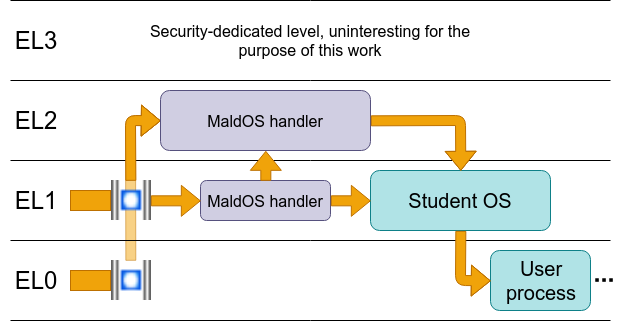
\includegraphics[scale=0.58]{execution_levels.png}
    }

    \begin{comment}
        La seconda parte seguita e' l'esecuzione di un processore ARMv8 si gestisce su 4 livelli, con una
        notevole semplificazione rispetto ai 9 della versione precedente.
        Gli studenti che sviluppano sul layer di astrazione sono interessati soltanto
        ai primi due, il livello non privilegiato per i processi (EL0) e quello
        elevato per il kernel(EL1).
        Il livello EL2 e' pensato per ospitare un hypervisor, ovvero un'entita' 
        che gestisca altri sistemi operativi virtualizzati. Idealmente quindi 
        il livello di astrazione dovrebbe vivere qui, ma non sempre e' conveniente.
        In generale l'hypervisor sarebbe pensato per virtualizzare interi sistemi
        operativi avendo un intero sistema operativo come host; questa situazione
        ha differenze lievi ma significative.
        Quando viene sollevato un interrupt di qualsiasi tipo MaldOS
        entra in gioco per primo, preparando il campo per il cambio di contesto.
        Alcune eccezioni salgono direttamente a EL2; altre rimangono a EL1 a seconda
        di quello che e' ritenuto piu' conveniente.
    \end{comment}
\end{frame}

\begin{frame}[fragile]
    \frametitle{Emulated Devices}
    \textbf{MaldOS} creates $\mu$MPS-style emulated devices with an ideal interface.
    Thanks to the mailbox interface the integration is seamless.

    \bigskip
    \begin{minipage}{0.49\textwidth}
        \begin{table}[]
            \begin{tabular}{|c|}
            \hline
            \rowcolor[HTML]{9B9B9B} 
            Virtual Disk device registers \\ \hline
            status register       \\ \hline
            command register      \\ \hline
            data 0 register       \\ \hline
            data 1 register       \\ \hline
            mailbox register      \\ \hline
            \end{tabular}
        \end{table}
    \end{minipage}
    \begin{minipage}{0.49\textwidth}
        \begin{table}[]
            \begin{tabular}{c}
            \hline
            \rowcolor[HTML]{9B9B9B} 
            \multicolumn{1}{|c|}{\cellcolor[HTML]{9B9B9B}EMMC device registers} \\ \hline
            \multicolumn{1}{|c|}{second argument register}                      \\ \hline
            \multicolumn{1}{|c|}{block size count register}                     \\ \hline
            \multicolumn{1}{|c|}{first argument register}                       \\ \hline
            \multicolumn{1}{|c|}{command register}                              \\ \hline
            \multicolumn{1}{|c|}{response registers (4)}                        \\ \hline
            \multicolumn{1}{|c|}{status register}                               \\ \hline
            \multicolumn{1}{|c|}{control register (2 of 3)}                     \\ \hline
            \multicolumn{1}{|c|}{interrupt register}                            \\ \hline
            \multicolumn{1}{|c|}{interrupt mask register}                       \\ \hline
            \multicolumn{1}{r}{... 11 more}                                    
            \end{tabular}
            \end{table}
    \end{minipage}

    \begin{comment}
        Il terzo aspetto e' l'emulazione di alcuni dispositivi. Il Raspberry Pi 3
        include troppe poche periferiche didatticamente interessanti: il controllore
        USB e' troppo complesso, l'interfaccia di rete e' nascosta dietro l'USB;
        rimangono soltanto periferiche di basso livello (UART, SPI, I2C), il 
        display HDMI e la scheda SD.
        Questi ultimi due vengono manipolati per offrire dispositivi emulati
        piu' approcciabili. Il livello di astrazione divide lo schermo in quattro
        ottenendo ulteriori terminali e considera alcuni file con nomi speciali
        sul file system come ulteriori dispositivi a blocchi, nastri e dischi.
        L'interfaccia per i dispositivi emulati riprende quella ideale usata
        da uMPS2, con un registro in piu' per confermare la ricezione della mailbox;
        lo studente scrive il comando in una locazione di memoria particolare, 
        che viene poi presa in gestione dal primo core.
        Il controllore della microSD, al contrario, richiederebbe di conoscere
        un complesso protocollo di comunicazione su piu' di 20 registri disorganizzati
        e con funzioni diverse.
    \end{comment}
\end{frame}

\begin{frame}[fragile]
    \frametitle{Virtual Memory}
    \vspace{-2cm}
    \begin{wrapfigure}{r}{0.65\textwidth}
        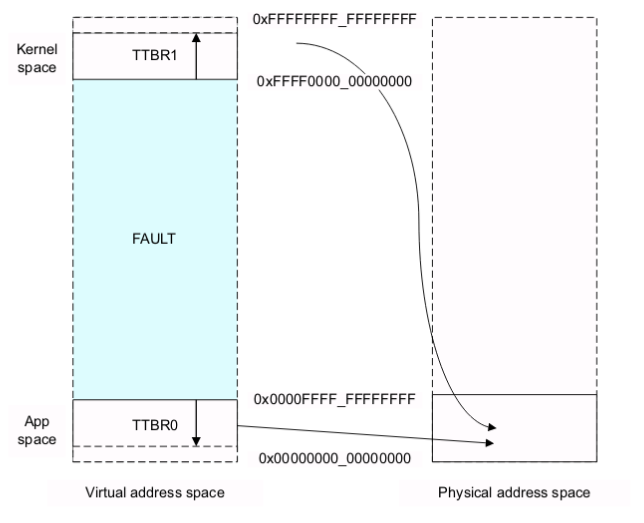
\includegraphics[scale=0.35]{ttbr.png}
    \end{wrapfigure}
    The ARMv8 MMU is remarkably flexible, so the virtual memory configuration is left
    mostly untouched.
    Students are assisted by changing page tables every time the kernel context
    switched in.

    \begin{comment}
        Quarto e ultimo aspetto, la memoria virtuale. Posto che la gestione di una
        MMU e' considerato uno sforzo inerentemente complesso, l'interfacciamento
        con il sistema rimane sostanzialmente intoccato.
        L'unica difficolta' sta nella configurazione iniziale: in generale, la
        memoria virtuale e' una funzionalita' che viene mantenuta sempre attiva;
        uno dei problemi iniziali dell'architettura MIPS era proprio l'impossibilita'
        di "spegnere" la MMU.
        Essendo in parte vicino al mondo embedded, l'architettura ARM permette
        di disattivare la traduzione di memoria; tuttavia rimane un meccanismo
        fortemente integrato nel sistema: esistono due registri, ttbr0 e ttbr1,
        che puntano a due tabelle delle pagine diverse; la discriminante per quale
        usare non e' pero' il livello di esecuzione (come sarebbe conveniente), 
        ma i due byte piu' significativi dell'indirizzo. Per usare una page table 
        diversa quindi il kernel deve apparire come caricato a un indirizzo di
        memoria inesistente, il che e' inconciliabile con una attivazione tardiva
        della MMU. Per risolvere questo problema gli handler degli interrupt scambiano
        i due registri TTBR0 e TTBR1 prima di passare il controllo al kernel,
        ottenendo l'impressione di page table legate al livello di esecuzione.
    \end{comment}
\end{frame}

\begin{frame}[plain,fragile]
    \frametitle{Qemu and Debugging}
    \makebox[\linewidth]{
        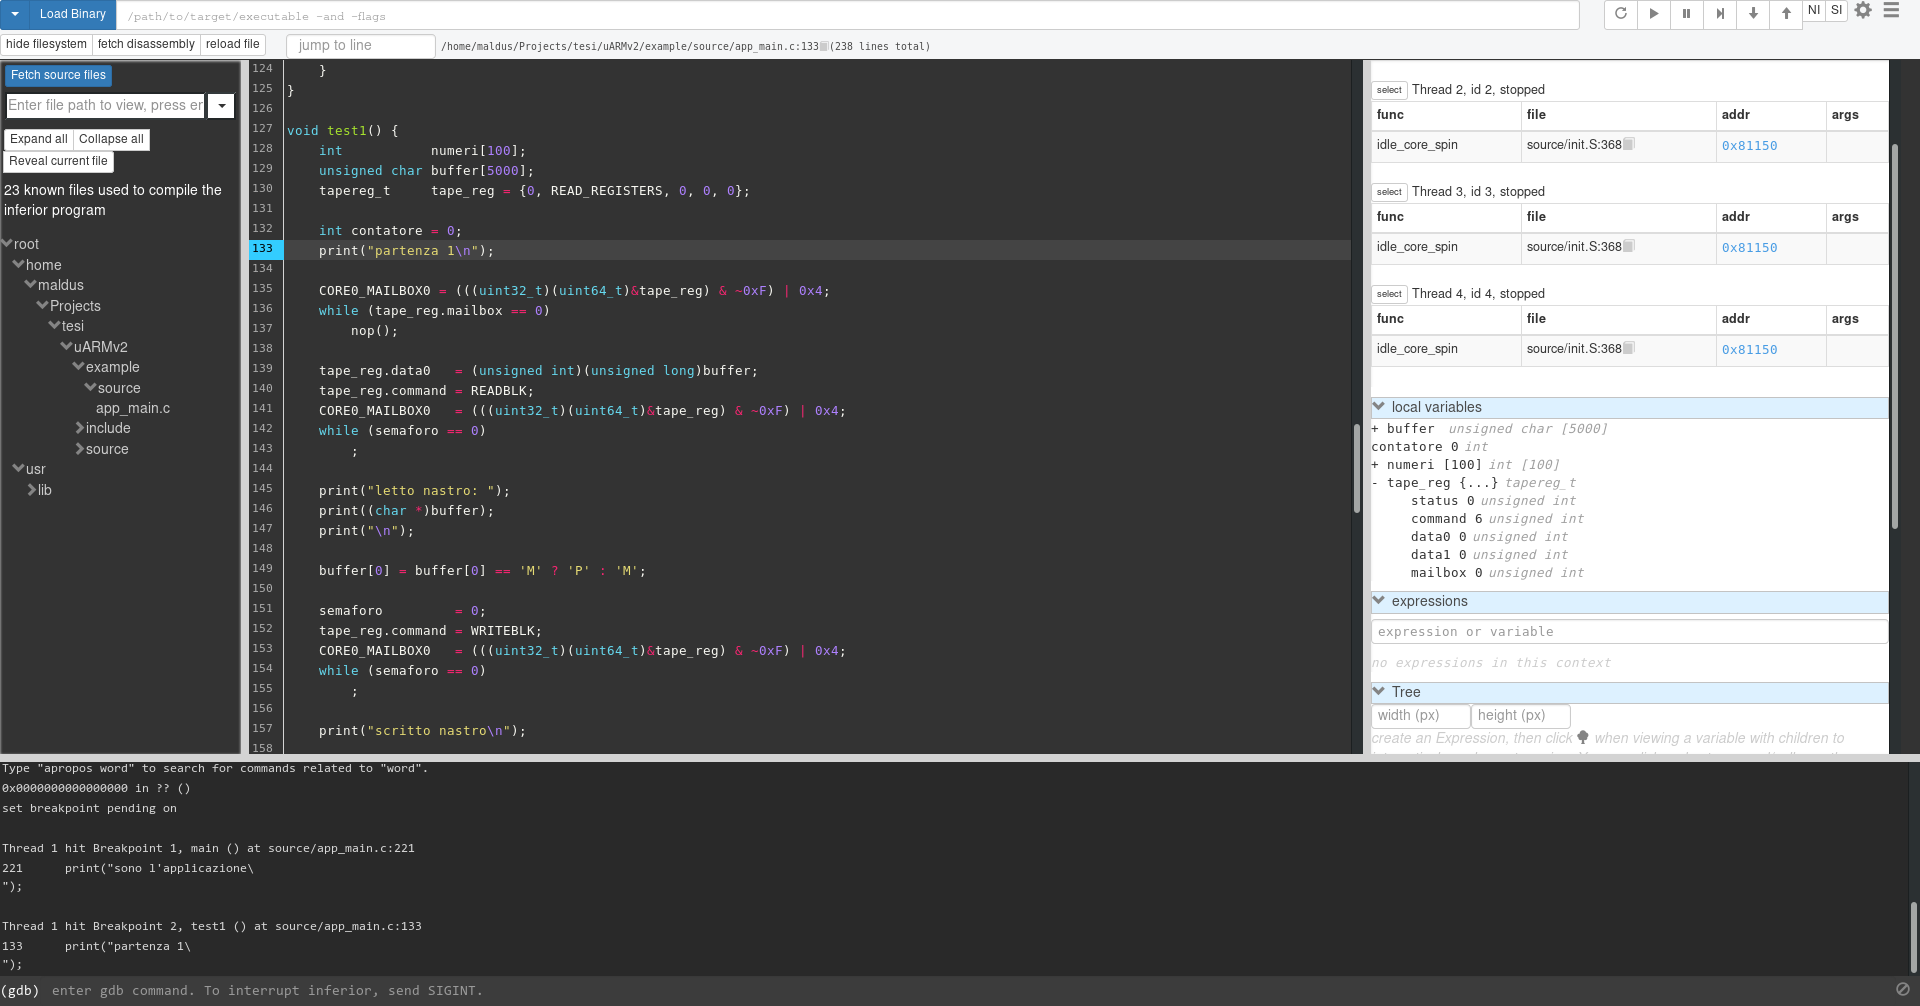
\includegraphics[width=12.5cm,height=8cm]{gdbgui.png}
    }

    \begin{comment}
        Mentre il kernel e' in esecuzione su Qemu puo' essere debuggato usando
        GDB. Non viene fornita un'interfaccia specializzata per il progetto, ma
        nel caso sarebbe relativamente semplice implementarne una: GDB mette a
        disposizione un interprete di comandi "macchina" proprio per
        poter costruire interfacce grafiche sofisticate. Per la durata di questo
        progetto e' stata usata GDBGUI, un tool Python che agisce da webserver
        e permette di debuggare tramite browser. Si puo' eseguire il codice passo
        per passo, ispezionare variabili, stabilire breakpoint, leggere la memoria
        e visualizzare separatamente i quattro core del processore.
    \end{comment}
\end{frame}

\end{document}